\section{Execution}
\label{sec:Execution}

The execution will be split up in different segments, so we can focus on the steps necessary to get the absorption spectrum of Rubidium.
During the entire runtime of the experiment everyone in the room needs to wear safety goggles!

\subsection{Setting up the laser}
\label{ssec:exe1}

Assuming the laser has already heaten up and reaches its optimum temperature we need to align the laser first.
For that you need to assemble the diode laser to the optical breadboard.
In its direction of emmitting we put the Rubidum absorption cell and behind it a photodiode detector to register the laserbeam.
Now we need to align the laser, so that its beam goes directly into the cell.
For that the laser is not visible for the human eye we need the IR Card to see its position. 
The orange circle area of the card emitts light if hit with the laserbeam. 
With this method you can locate the laser, although it is invisible.
Put the TV camera in front of the card, so that you can observe the emitted light clearly.
Your setup should look like in \autoref{fig:part1}.
\begin{figure}
    \centering
    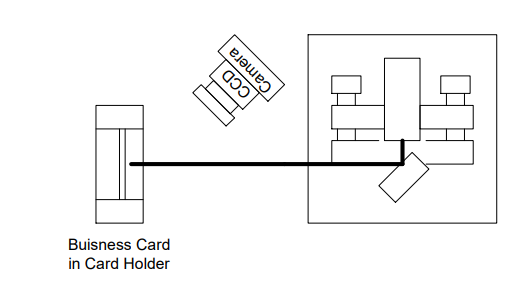
\includegraphics[width=0.5\textwidth]{images/part1.png}
    \caption{Setup for lining up the laser \cite{V60}}
    \label{fig:part1}
\end{figure}
Now we increase the current of the laser, until spreckles are visible on the card. 
The laser is now lasing. 
Take a picture of the monitor where the laser is lasing and one where its not.

Our pictures are shown in \autoref{fig:lasing}.
\begin{figure}
    \centering
    \begin{subfigure}[t]{0.3\textwidth}
        \centering
        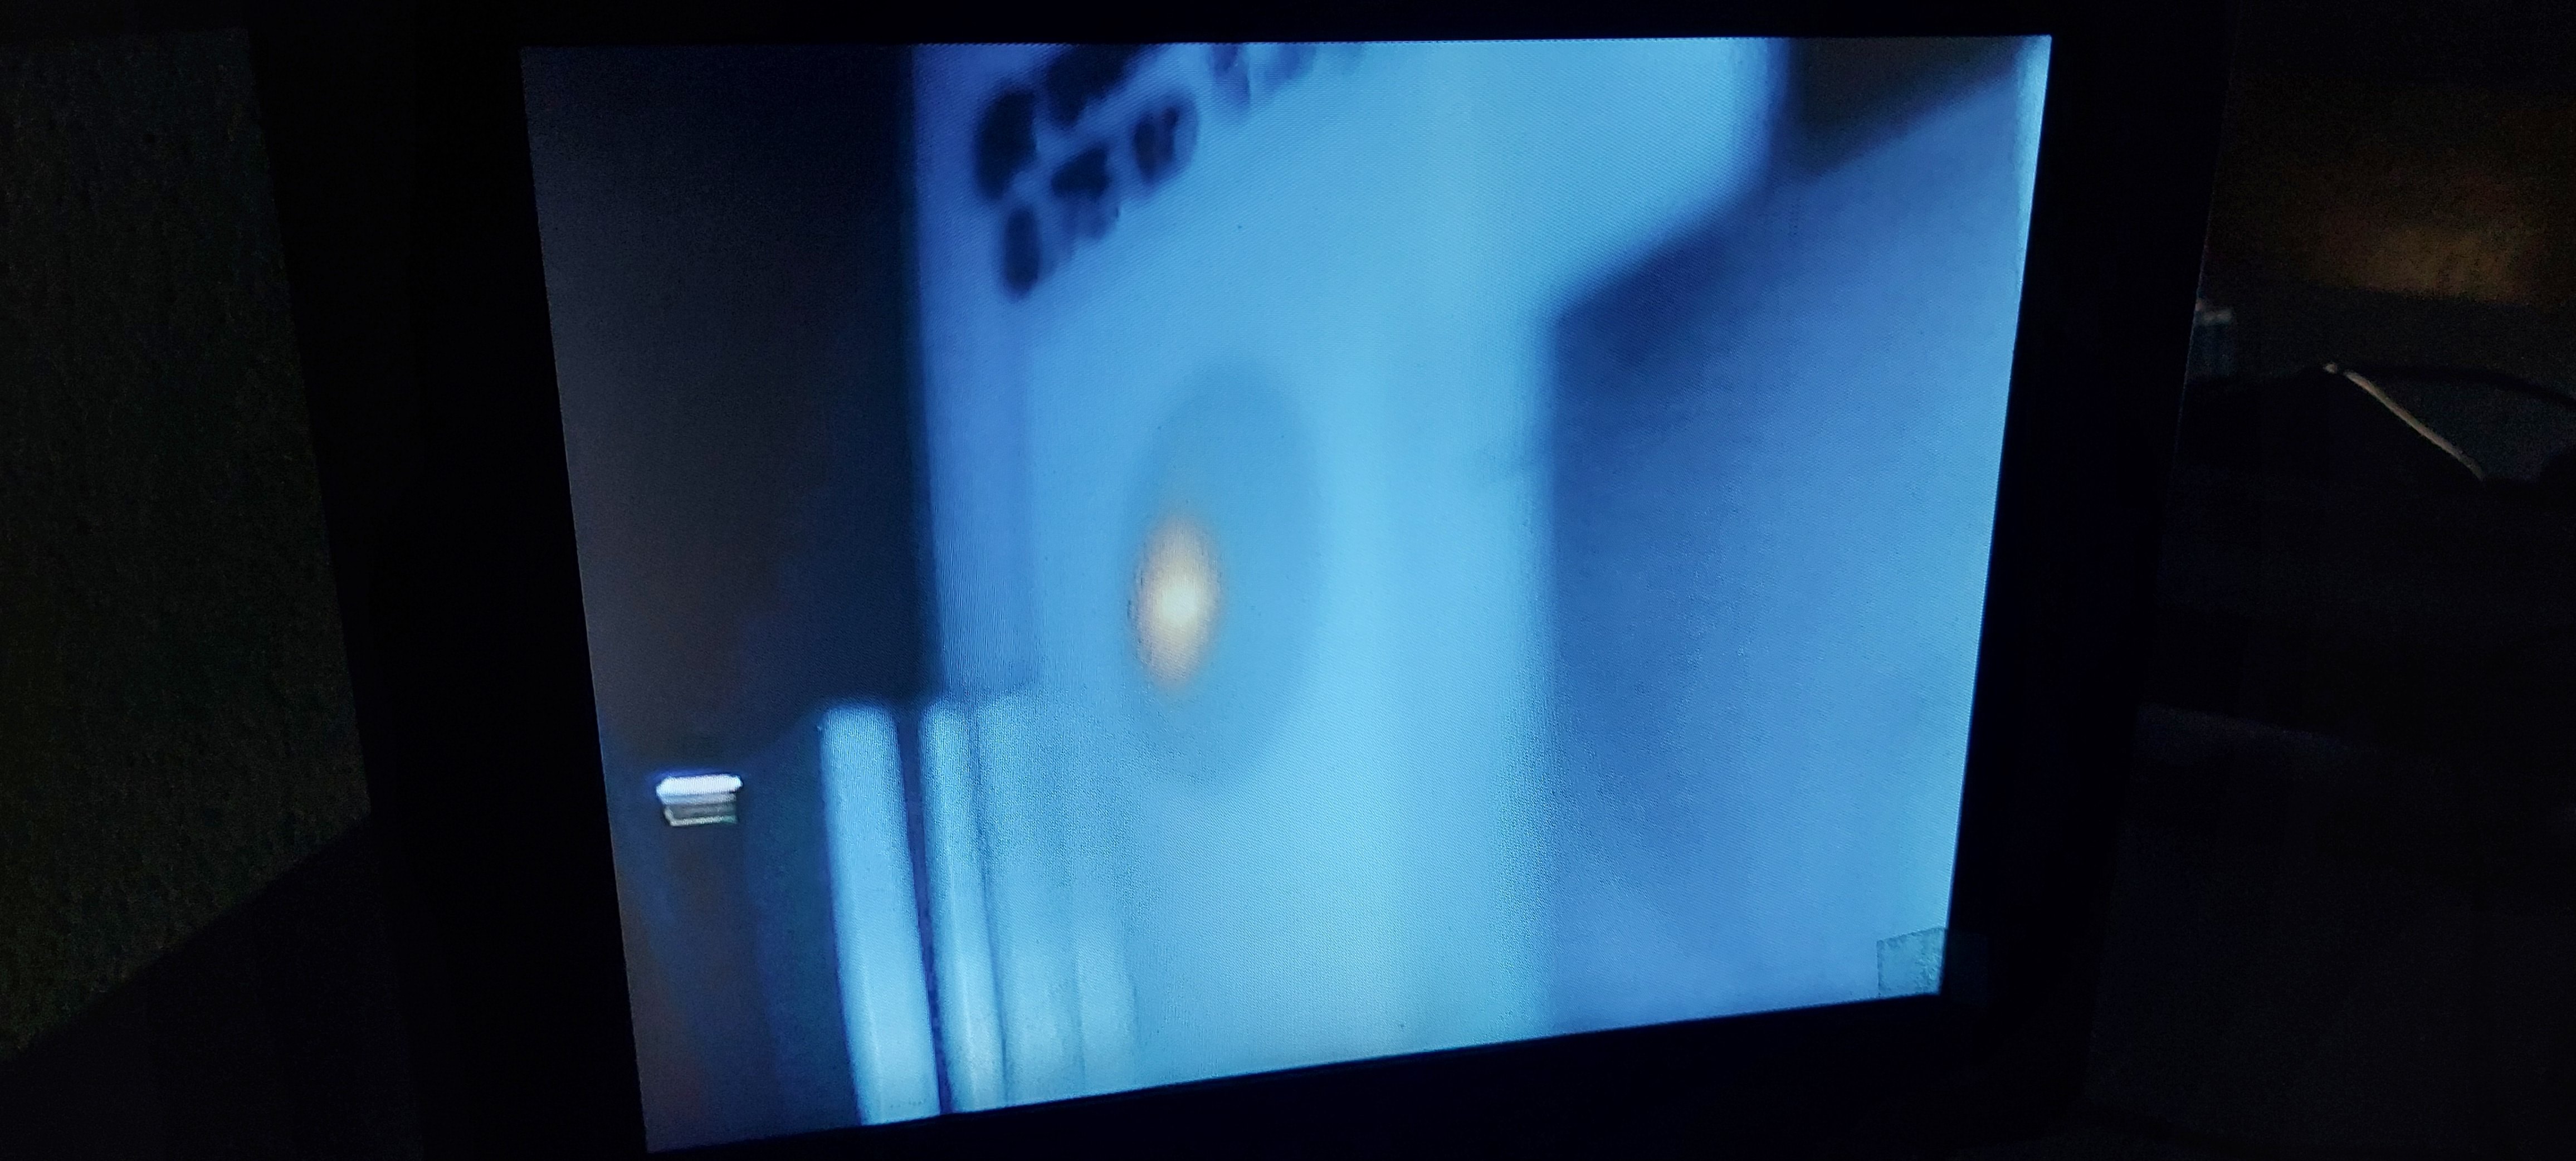
\includegraphics[width=\textwidth]{images/photo_not_lasing.jpg}
        \caption{Picture of the laser before lasing}
        \label{fig:notlase}
    \end{subfigure}
    \begin{subfigure}[t]{0.3\textwidth}
        \centering
        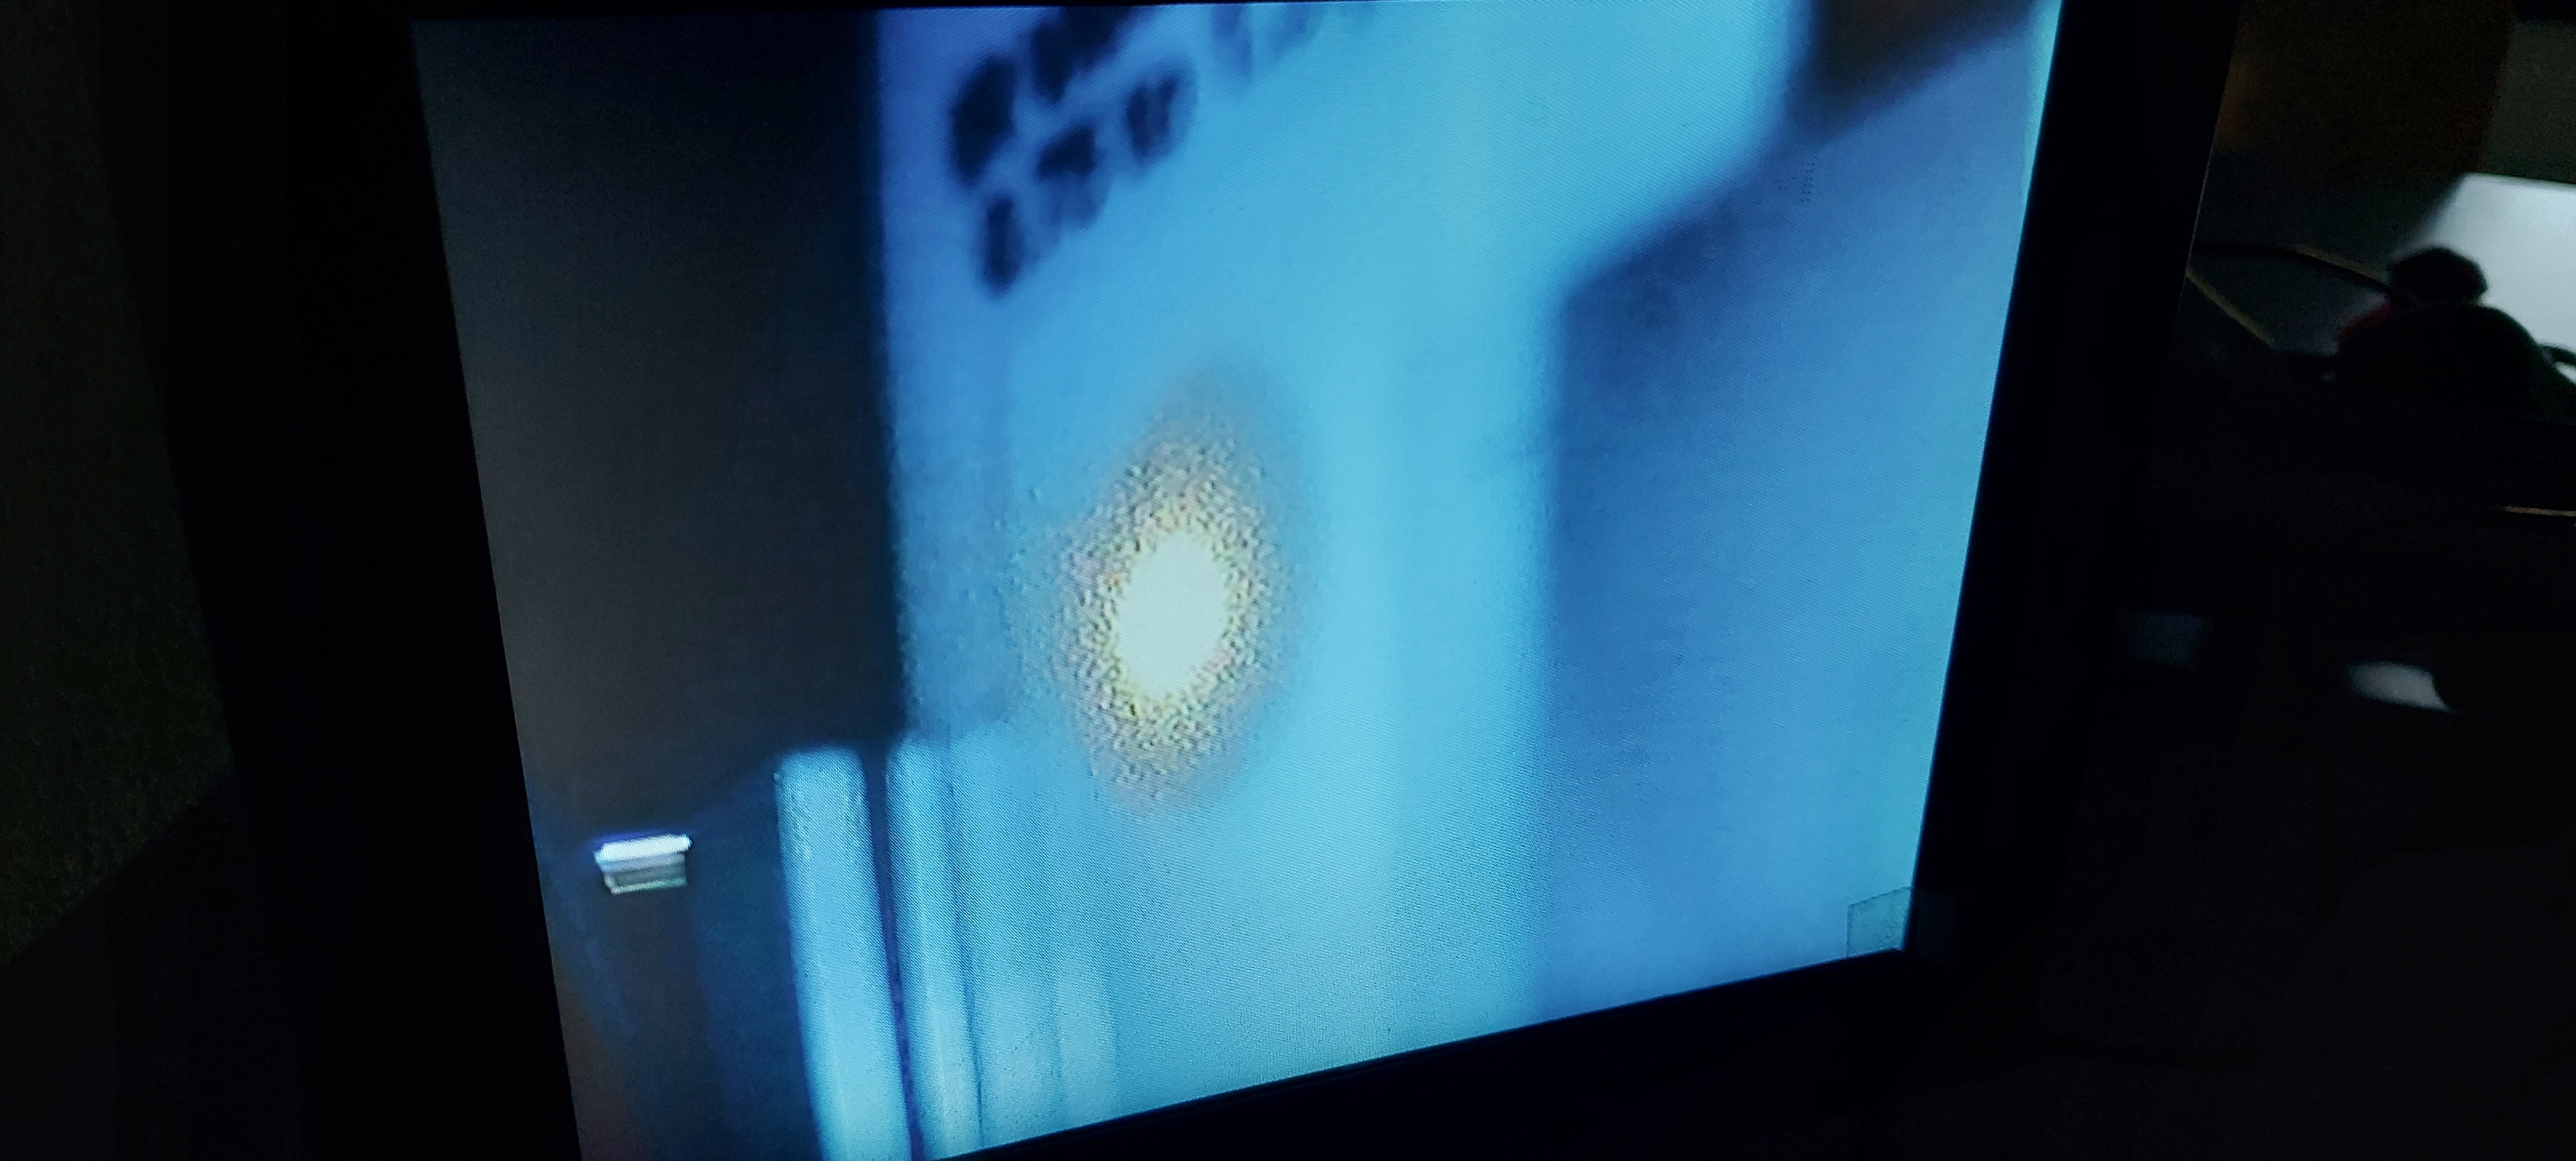
\includegraphics[width=\textwidth]{images/photo_lasing.jpg}
        \caption{Picture of the laser lasing}
        \label{fig:lase}
    \end{subfigure}
    \caption{Our picutures made for this experiment}
    \label{fig:lasing}
\end{figure}

\subsection{Calibration of the absorption wavelength}
\label{ssec:exe2}

First we take the IR Card away and let the laser go into the Rubidium cell. 
Then you rearrange the camera, so it looks directly in the side hole of the cell. 
For optimum results you should also dim the lights, so that no other light source may influence the photodiode.
You also need to reduce the intesity of the laser or your photodiode will not show the wanted result, so you put different filters right after the laser.
Now you need to set up the oscilloscope for the calibration, for that you need to recreate the setup in \autoref{fig:osci1}.
\begin{figure}
    \centering
    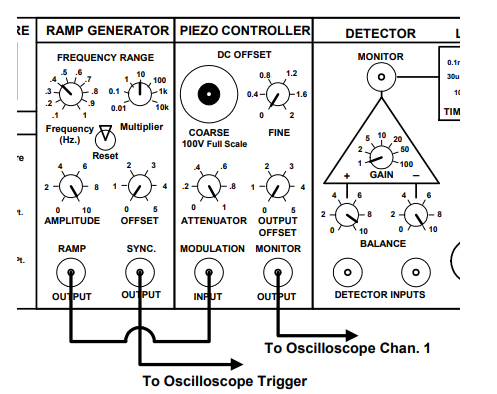
\includegraphics[width=0.5\textwidth]{images/generator.png}
    \caption{Setup of the oscilloscope for the calibration \cite{V60}}
    \label{fig:osci1}
\end{figure}
After that your experiment should look like in \autoref{fig:part2}.
\begin{figure}
    \centering
    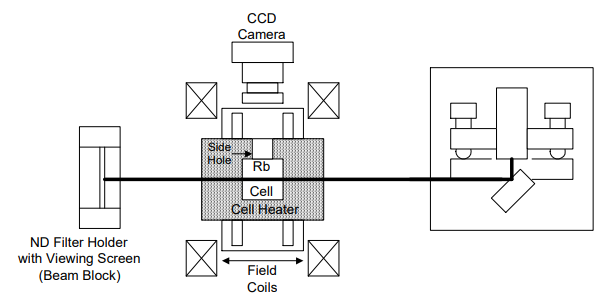
\includegraphics[width=0.5\textwidth]{images/part2.png}
    \caption{Experiment when calibrating the absorption wavelength \cite{V60}}
    \label{fig:part2}
\end{figure}
Set the ramp generator frequency to $\SI{10}{\hertz}$ and calibrate the settings so that the ramp generator produses a large-amplitude triangle wave.
Then you can start adjusting the laser current of the diode laser.
When the Rubidium cell stars emitting light in a consistant strengh you found the right frequency.
Take a photo of the camera monitore.

The one we took is presented in \autoref{fig:leucht}.
\begin{figure}
    \centering
    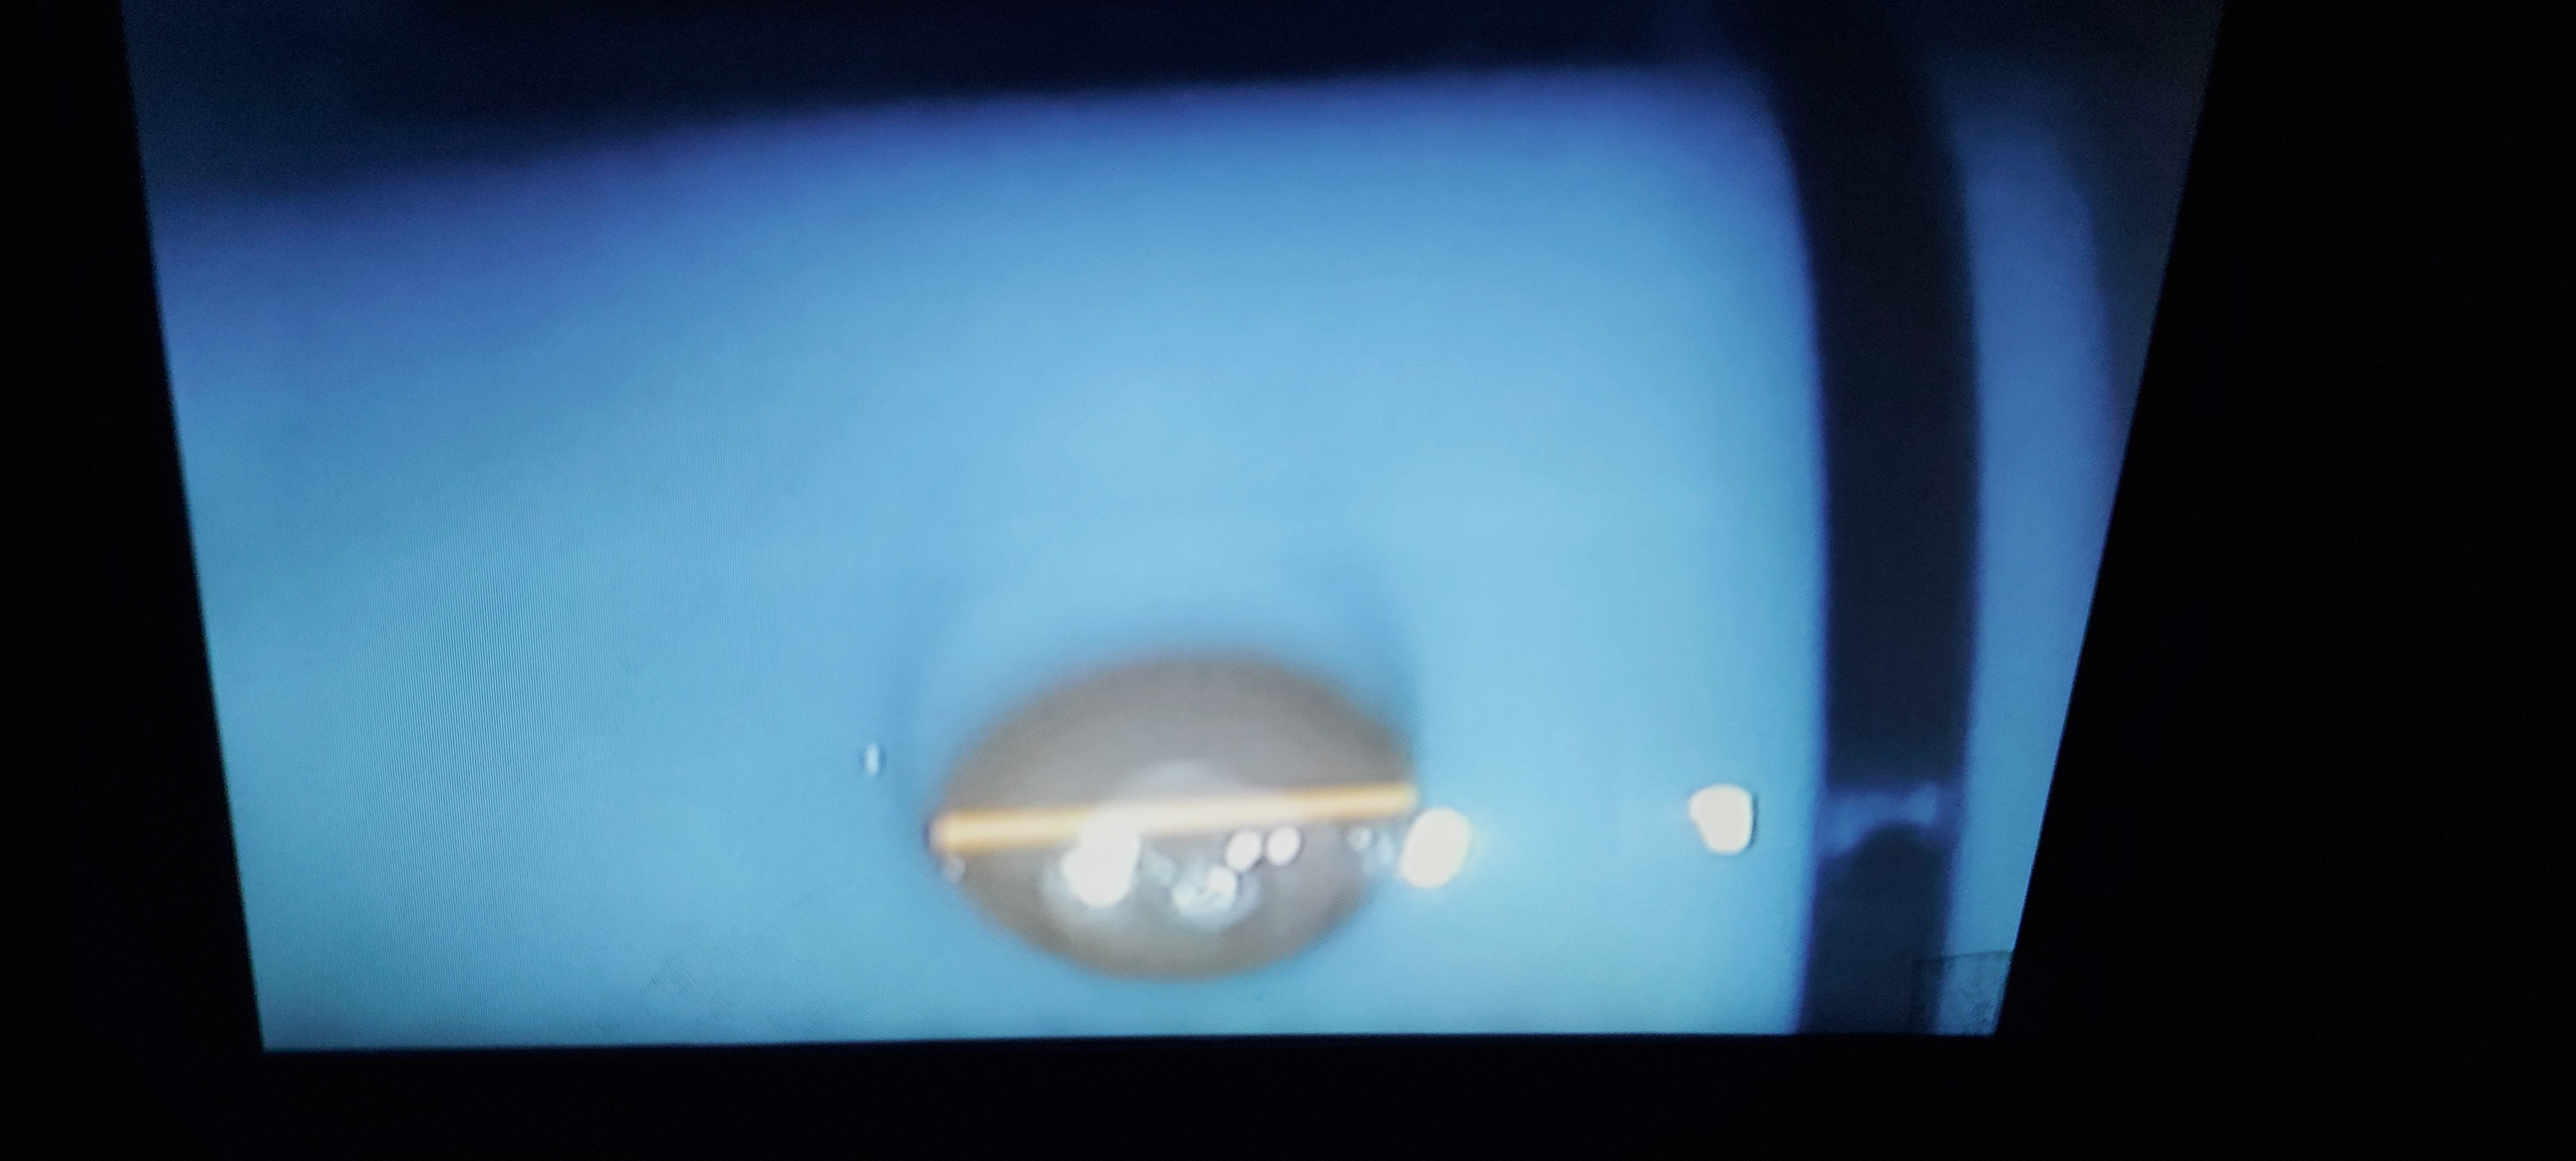
\includegraphics[width=0.5\textwidth]{images/photo_fluorescence.jpg}
    \caption{Photo of the fluorescence in the rubidium cell}
    \label{fig:leucht}
\end{figure}

On the oscilloscope you should now see mode hops.
In the next part we will try to eliminate them through simultaneous usage of current and piezo modulation.

\subsection{The absorption spectrum}
\label{ssec:exe3}

To get rid of the mode hops and to see a good picture of the absorption spectrum we change the setup of the experiment. 
First of we rearrange the cables on the oscilloscope to what is shown in \autoref{fig:osci2}.
\begin{figure}
    \centering
    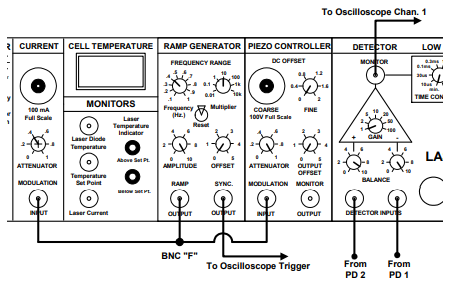
\includegraphics[width=0.5\textwidth]{images/generator2.png}
    \caption{Setup of the oscilloscope for the absorption spectrum \cite{V60}}
    \label{fig:osci2}
\end{figure}
Now we want do produce a better picture of the spectrum. 
You turn the ramp generator amplitude up to maximum and follow that up with turning up the current attenuator knob.
You should be able to use all the knobs and calibrations to make a picture like in \autoref{fig:osci3}, but here it is inverted.
\begin{figure}
    \centering
    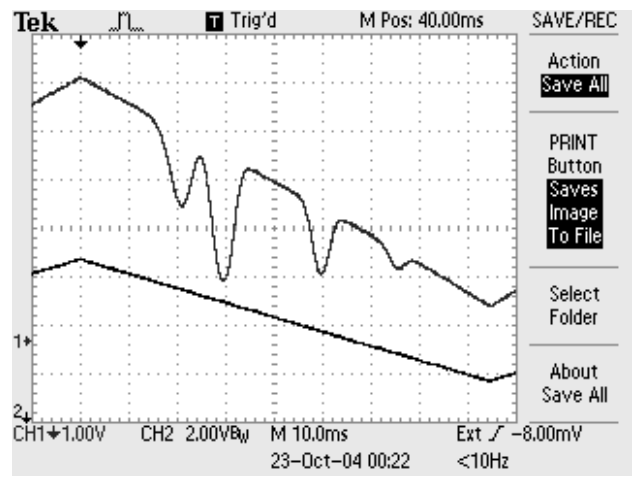
\includegraphics[width=0.5\textwidth]{images/oszi.png}
    \caption{Picture of the absorption lines without mode hops \cite{V60}}
    \label{fig:osci3}
\end{figure}
Cleary this is not the optimal figure.
The scan of the laser intensity and the laser frequency are scanned together here, but we can correct that.
We add a second photodiode on the optical breadboard.
Put a 50/50 Beam splitter in front of the Rubidium cell and place the second photodiode in its path, like shown in \autoref{fig:part3}.
\begin{figure}
    \centering
    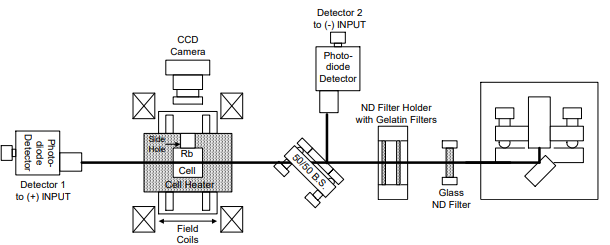
\includegraphics[width=0.5\textwidth]{images/part3.png}
    \caption{Final setup of the optical breadboard \cite{V60}}
    \label{fig:part3}
\end{figure}
After final adjustments the final figure on the oscilloscope should be spectrum shown in \autoref{fig:osci4}.
\begin{figure}
    \centering
    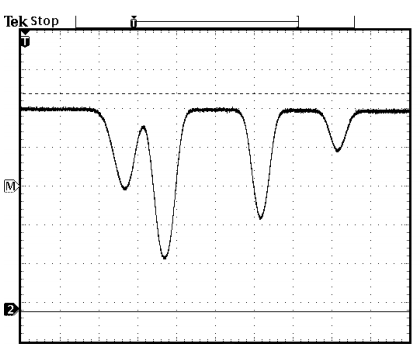
\includegraphics[width=0.5\textwidth]{images/oszi2.png}
    \caption{Inverted absorption spectrum of rubidium \cite{V60}}
    \label{fig:osci4}
\end{figure}
If we compare our picture in \autoref{fig:spektrum} with the theoretical one, its fair to say, that the recording of the absorption spectrum was successfull.
\begin{figure}
    \centering
    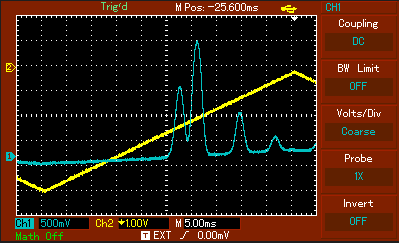
\includegraphics[width=0.5\textwidth]{images/spektrum.png}
    \caption{Our not inverted absorption spectrum of rubidium}
    \label{fig:spektrum}
\end{figure}